\documentclass[color=usenames,dvipsnames]{beamer}

\mode<presentation> {

\usetheme{Madrid}

\usepackage{multirow}

\usepackage{tikz}
\usetikzlibrary{shapes.geometric, arrows}

\definecolor{ERC1}{HTML}{C72321}
\definecolor{ERC2}{HTML}{861719}
\definecolor{ERC3}{HTML}{FBD7A9}
\definecolor{ERC4}{HTML}{BA9F7C}
\definecolor{ERC5}{HTML}{7A6952}
\definecolor{ERC6}{HTML}{6E9B9E}
\definecolor{ERC7}{HTML}{0D8085}
\definecolor{ERC8}{HTML}{19484C}
\definecolor{ERC9}{HTML}{F0C320}
\definecolor{ERC10}{HTML}{AF8F19}


\tikzstyle{startstop} = [rectangle, rounded corners, minimum width=3cm, minimum height=1cm,text centered, draw=black, fill=ERC8]
\tikzstyle{io} = [trapezium, trapezium left angle=70, trapezium right angle=110, minimum width=3cm, minimum height=1cm, text centered, draw=black, fill=ERC7]
\tikzstyle{process} = [rectangle, minimum width=3cm, minimum height=1cm, text centered, draw=black, fill=ERC9]
\tikzstyle{decision} = [diamond, minimum width=3cm, minimum height=1cm, text centered, draw=black, fill=ERC10]
\tikzstyle{arrow} = [thick,->,>=stealth]


\setbeamercolor{palette primary}{bg=ERC1,fg=white}
\setbeamercolor{palette secondary}{bg=ERC2,fg=white}
\setbeamercolor{palette tertiary}{bg=ERC3,fg=white}
\setbeamercolor{palette quaternary}{bg=ERC4,fg=white}
\setbeamercolor{structure}{fg=ERC5} % itemize, enumerate, etc
\setbeamercolor{section in toc}{fg=ERC6} % TOC sections

%gets rid of bottom navigation bars
\setbeamertemplate{footline}[frame number]{}

%gets rid of bottom navigation symbols
\setbeamertemplate{navigation symbols}{}

%gets rid of footer
%will override 'frame number' instruction above
%comment out to revert to previous/default definitions
\setbeamertemplate{footline}{}

% Override palette coloring with secondary
%\setbeamercolor{subsection in head/foot}{bg=UBCgrey,fg=white}


%\usecolortheme{lily}
\useoutertheme{infolines}

}


\usepackage{booktabs} 
\usepackage{tikz}


% Thin fonts
\usepackage{cmbright}
\usepackage[T1]{fontenc}

\definecolor{dark_grey}{gray}{0.5}
%\setbeamercolor{normal text}{fg=dark_grey,bg=white}
\setbeamertemplate{navigation symbols}{}

%\setbeamercolor*{palette primary}{fg=gray!100,bg=gray!10}
%\setbeamercolor*{palette quaternary}{fg=gray!100,bg=gray!10}
%\setbeamercolor*{palette secondary}{fg=gray!100,bg=gray!20}
%\setbeamercolor*{palette tertiary}{fg=gray!100,bg=gray!10}
%\setbeamercolor*{navigation symbols}{fg=white,bg=white}
\usefonttheme{default}


\setbeamertemplate{blocks}[rounded][shadow=false]
%\setbeamercolor{block title}{bg=gray!10}
%\setbeamercolor{block body}{fg=gray,bg=gray!10}
%\setbeamercolor{frametitle}{fg=}

\setbeamertemplate{frametitle}[default][center]

\setbeamertemplate{itemize items}[default]
\setbeamertemplate{enumerate items}[default]

\newcommand{\F}{\mathbb{F}}

\setbeamertemplate{title page}[default][colsep=-4bp,rounded=true]

\title[Workshop - Machine Learning]{ Don't believe the hype? A hands-on introduction to machine-learning in Python - Part III.2}
\subtitle{Open Workshops on Computer Based Systems Modelling}

\author{Johannes Schmidt, Johann Baumgartner}
\institute{Institute for Sustainable Economic Development, BOKU, Vienna}
\date{7.05.2019}

\begin{document}

{
\usebackgroundtemplate{
 \begin{picture}(320,315)
 \hspace{6.9cm}
   
\includegraphics[width=0.7\linewidth]{../figures/refuel_logo_with_text.png}
 \end{picture}
 }


\begin{frame}

\maketitle



\end{frame}
}
% Uncomment these lines for an automatically generated outline.
%\begin{frame}{Outline}
%  \tableofcontents
%\end{frame}
%\subsection{Mathematics}
\begin{frame}
\frametitle{Contents}
\begin{itemize}
	\item The Q-learning algorithm
	\item A very simple example calculated by hand
	\item A simple example in python
\end{itemize}

\end{frame}

\begin{frame}{The Q-learning algorithm in a nutshell}
\framesubtitle{Which action to pick?}
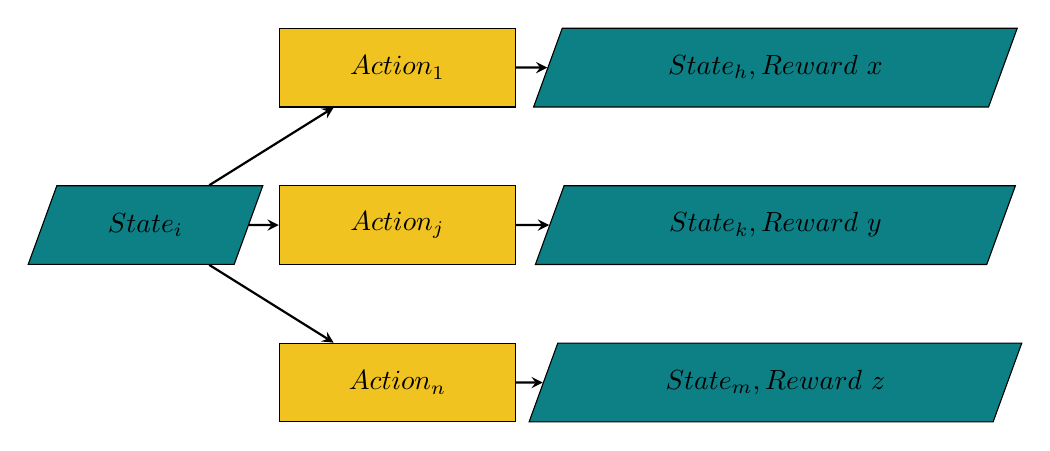
\begin{tikzpicture}[node distance=2cm]

%\node (Start) [startstop] {Start};

\node (si) [io] {$State_i$};

\node (a1) [process, right of=si, xshift=1.2cm, yshift=2cm] {$Action_1$};
\node (aj) [process, right of=si, xshift=1.2cm] {$Action_j$};
\node (an) [process, right of=si, xshift=1.2cm, yshift=-2cm] {$Action_n$};

\node (sip1) [io, right of=a1, xshift=2.8cm] {$State_{h}, Reward\ x$};
\node (sip2) [io, right of=aj, xshift=2.8cm] {$State_{k}, Reward\ y$};
\node (sip3) [io, right of=an, xshift=2.8cm] {$State_{m}, Reward\ z$};



\draw [arrow] (si) -- (a1);
\draw [arrow] (si) -- (aj);
\draw [arrow] (si) -- (an);

\draw [arrow] (a1) -- (sip1);
\draw [arrow] (aj) -- (sip2);
\draw [arrow] (an) -- (sip3);

\end{tikzpicture}
\end{frame}


\begin{frame}{The Q-Table}
\framesubtitle{The Q-Table is updated in a learning by doing approach}

Q-Updating rule introduced 1989 by Watson. Updates Q-Table according to current rewards and expected future rewards\\

$q^{new}(s_t,a_t)=(1-\alpha)q(s_t,a_t) + \alpha (r_t + \gamma \max\limits_{a} q(s_{t+1},a))$\\

$\alpha$ is learning rate, $\gamma$ is discount rate\\
$r_t$ is reward, $s_t$ is state, $a_t$ is action\\

\begin{table}
	\begin{tabular}{lllll}
		 \multicolumn{4}{c}{Actions}\\
\multirow{4}{*}{States}		& $q_{s_1,a_1}$ & $q_{s_1,a_2}$ & $q_{s_1,a_3}$  & $q_{s_1,a_4}$\\
							& $q_{s_2,a_1}$ & $q_{s_2,a_2}$ & $q_{s_2,a_3}$  & $q_{s_2,a_4}$\\
							& $q_{s_3,a_1}$ & $q_{s_3,a_2}$ & $q_{s_3,a_3}$  & $q_{s_3,a_4}$\\
							& $q_{s_4,a_1}$ & $q_{s_4,a_2}$ & $q_{s_4,a_3}$  & $q_{s_4,a_4}$\\
	\end{tabular}
\end{table}

\end{frame}




{
\usebackgroundtemplate{
 \begin{picture}(320,315)
 \hspace{6.9cm}
   
\includegraphics[width=0.7\linewidth]{../figures/refuel_logo_with_text.png}
 \end{picture}
 }


\begin{frame}
\frametitle{Thank you!}
\begin{block}{
 For updates on the project, check \textbf{refuel.world}\\
 For source-code, check \textbf{github.com/joph/MachineLearningCourse}\\
 
		mail: johannes.schmidt@boku.ac.at\\

}
\end{block}

\vspace{2.5 cm}


\end{frame}

}


\end{document} 